\chapter{Psalm 16}

\begin{figure}
  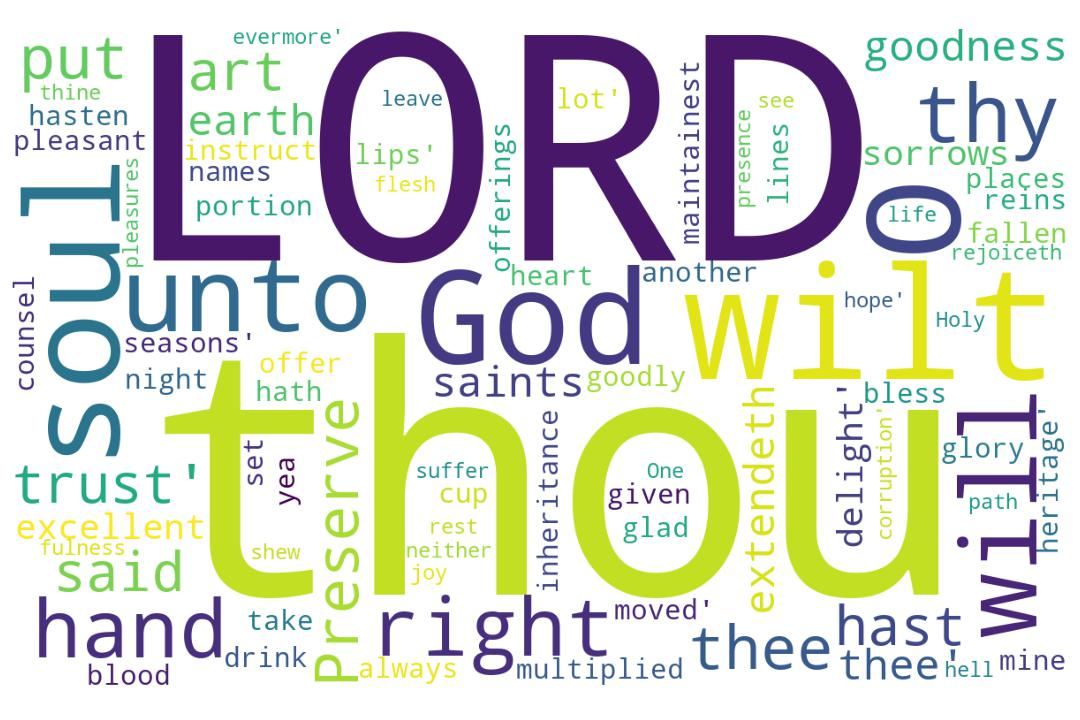
\includegraphics[width=\linewidth]{19OT-Psalms/Psalm16-WordCloud.jpg}
  \caption{Psalm 16 Word Cloud}
  \label{fig:Psalm 16 word Cloud}
\end{figure}



\marginpar{\scriptsize \centering \fcolorbox{bone}{lime}{\textbf{CONTRASTS}}\\ (Psalm 16:1--11) \begin{compactenum}[I.][8]
	\item Thirteen \textbf{Possession} \index[scripture]{Psalms!Psa 016:01}(Psa 16:1)
	\begin{compactenum}[A.]
	    \item My \textbf{trust} \index[scripture]{Psalms!Psa 016:01}(Psa 16:1)
	    \item My \textbf{soul} \index[scripture]{Psalms!Psa 016:02}(Psa 16:2)
	    \item My \textbf{Lord} \index[scripture]{Psalms!Psa 016:02}(Psa 16:2)
	    \item My \textbf{goodness} \index[scripture]{Psalms!Psa 016:02}(Psa 16:2)
	    \item My \textbf{delight} \index[scripture]{Psalms!Psa 016:03}(Psa 16:3)
	    \item My \textbf{lips} \index[scripture]{Psalms!Psa 016:04}(Psa 16:4)
	    \item My \textbf{cup} \index[scripture]{Psalms!Psa 016:05}(Psa 16:5)
	    \item My \textbf{lot} \index[scripture]{Psalms!Psa 016:05}(Psa 16:5)
	    \item My \textbf{right hand} \index[scripture]{Psalms!Psa 016:08}(Psa 16:8)
	    \item My \textbf{heart} \index[scripture]{Psalms!Psa 016:09}(Psa 16:9)
	    \item My \textbf{glory} \index[scripture]{Psalms!Psa 016:09}(Psa 16:9)
	    \item My \textbf{flesh} \index[scripture]{Psalms!Psa 016:09}(Psa 16:9)
	    \item My \textbf{soul} \index[scripture]{Psalms!Psa 016:10}(Psa 16:10)
	\end{compactenum}
	\item One \textbf{Provision} (thine Holy One) \index[scripture]{Psalms!Psa 016:10}(Psa 16:10)
	\item One \textbf{Promise} (mine inheritance) \index[scripture]{Psalms!Psa 016:05}(Psa 16:5)
\end{compactenum}}

\footnote{\textcolor[cmyk]{0.99998,1,0,0}{\hyperlink{TOC}{Return to end of Table of Contents.}}}\footnote{\href{https://www.audioverse.org/english/audiobibles/books/ENGKJV/O/Ps/1}{\textcolor[cmyk]{0.99998,1,0,0}{Psalms Audio}}}\textcolor[cmyk]{0.99998,1,0,0}{Michtam of David.}\\
\\
\textcolor[cmyk]{0.99998,1,0,0}{Preserve me, O God: for in thee do I put \fcolorbox{bone}{lime}{my trust}.}\footnote{\textbf{Psalm 17:5,8} - Hold up my goings in thy paths, that my footsteps slip not. [8] Keep me as the apple of the eye, hide me under the shadow of thy wings,}\footnote{\textbf{Psalm 31:23} - O love the LORD, all ye his saints: for the LORD preserveth the faithful, and plentifully rewardeth the proud doer.}\footnote{\textbf{Psalm 37:28} - For the LORD loveth judgment, and forsaketh not his saints; they are preserved for ever: but the seed of the wicked shall be cut off.}\footnote{\textbf{Psalm 56:1} - Be merciful unto me, O God: for man would swallow me up; he fighting daily oppresseth me.}\footnote{\textbf{Psalm 60:1} - O God, thou hast cast us off, thou hast scattered us, thou hast been displeased; O turn thyself to us again.}\footnote{\textbf{Psalm 97:10} - Ye that love the LORD, hate evil: he preserveth the souls of his saints; he delivereth them out of the hand of the wicked.}\footnote{\textbf{Psalm 116:6} - The LORD preserveth the simple: I was brought low, and he helped me.}\footnote{\textbf{Proverb 2:8} - He keepeth the paths of judgment, and preserveth the way of his saints.}\footnote{\textbf{Isaiah 26:3-4} - Thou wilt keep him in perfect peace, whose mind is stayed on thee: because he trusteth in thee. [4] Trust ye in the LORD for ever: for in the LORD JEHOVAH is everlasting strength:}\footnote{\textbf{2 Corinthians 1:9} - But we had the sentence of death in ourselves, that we should not trust in ourselves, but in God which raiseth the dead:}\footnote{\textbf{2 Timothy 1:12} - For the which cause I also suffer these things: nevertheless I am not ashamed: for I know whom I have believed, and am persuaded that he is able to keep that which I have committed unto him against that day.}
[2] \textcolor[cmyk]{0.99998,1,0,0}{\emph{O} \fcolorbox{bone}{lime}{\emph{my} \emph{soul}}, thou hast said unto the LORD, Thou \emph{art} \fcolorbox{bone}{lime}{my Lord}: \fcolorbox{bone}{lime}{my goodness} \emph{extendeth} not to thee;}\footnote{\textbf{Job 22:2-3} - Can a man be profitable unto God, as he that is wise may be profitable unto himself? [3] Is it any pleasure to the Almighty, that thou art righteous? or is it gain to him, that thou makest thy ways perfect?}\footnote{\textbf{Job 35:7-8} - If thou be righteous, what givest thou him? or what receiveth he of thine hand? [8] Thy wickedness may hurt a man as thou art; and thy righteousness may profit the son of man.}\footnote{\textbf{John 20:28} - And Thomas answered and said unto him, My Lord and my God.}
[3] \textcolor[cmyk]{0.99998,1,0,0}{\emph{But} to the saints that \emph{are} in the earth, and \emph{to} the excellent, in whom \emph{is} all \fcolorbox{bone}{lime}{my delight}.}\footnote{\textbf{Psalm 30:4} - Sing unto the LORD, O ye saints of his, and give thanks at the remembrance of his holiness.}
[4] \textcolor[cmyk]{0.99998,1,0,0}{Their sorrows shall be multiplied \emph{that} hasten \emph{after} another \emph{god}: their drink offerings of blood will I not offer, nor take up their names into \fcolorbox{bone}{lime}{my lips}.}\footnote{\textbf{Psalm 32:10} - Many sorrows shall be to the wicked: but he that trusteth in the LORD, mercy shall compass him about.}\footnote{\textbf{Psalm 97:7} - Confounded be all they that serve graven images, that boast themselves of idols: worship him, all ye gods.}\footnote{\textbf{Jonah 2:8} - They that observe lying vanities forsake their own mercy.}\footnote{\textbf{Genesis 35:14} - And Jacob set up a pillar in the place where he talked with him, even a pillar of stone: and he poured a drink offering thereon, and he poured oil thereon.}
[5] \textcolor[cmyk]{0.99998,1,0,0}{The LORD \emph{is} the portion of mine inheritance and of \fcolorbox{bone}{lime}{my cup}: thou maintainest \fcolorbox{bone}{lime}{my lot}.}\footnote{\textbf{Psalm 73:26} - My flesh and my heart faileth: but God is the strength of my heart, and my portion for ever.}\footnote{\textbf{Psalm 119:57} - Thou art my portion, O LORD: I have said that I would keep thy words.}\footnote{\textbf{Psalm 142:5} - I cried unto thee, O LORD: I said, Thou art my refuge and my portion in the land of the living.}\footnote{\textbf{Deuteronomy 32:9} - For the LORD'S portion is his people; Jacob is the lot of his inheritance.}\footnote{\textbf{Jeremiah 10:16} - The portion of Jacob is not like them: for he is the former of all things; and Israel is the rod of his inheritance: The LORD of hosts is his name.}\footnote{\textbf{Lamentations 3:24} - The LORD is my portion, saith my soul; therefore will I hope in him.}
[6] \textcolor[cmyk]{0.99998,1,0,0}{The lines are fallen unto me in pleasant \emph{places}; yea, I have a goodly heritage.}
[7] \textcolor[cmyk]{0.99998,1,0,0}{I will bless the LORD, who hath given me counsel: my reins also instruct me in the night seasons.}
[8] \textcolor[cmyk]{0.99998,1,0,0}{I have set the LORD always before me: because \emph{he} \emph{is} at \fcolorbox{bone}{lime}{my right hand}, I shall not be moved.}
[9] \textcolor[cmyk]{0.99998,1,0,0}{Therefore \fcolorbox{bone}{lime}{my heart} is glad, and \fcolorbox{bone}{lime}{my glory} rejoiceth: \fcolorbox{bone}{lime}{my flesh} also shall rest in hope.}
[10] \textcolor[cmyk]{0.99998,1,0,0}{For thou wilt not leave \fcolorbox{bone}{lime}{my soul} in hell; neither wilt thou suffer thine Holy One to see corruption.}\footnote{\textbf{Acts 2:27, 31} - Because thou wilt not leave my soul in hell, neither wilt thou suffer thine Holy One to see corruption. [31] He seeing this before spake of the resurrection of Christ, that his soul was not left in hell, neither his flesh did see corruption.}\footnote{\textbf{Acts 13:34-37} - And as concerning that he raised him up from the dead, now no more to return to corruption, he said on this wise, I will give you the sure mercies of David. [35] Wherefore he saith also in another psalm, Thou shalt not suffer thine Holy One to see corruption. [36] For David, after he had served his own generation by the will of God, fell on sleep, and was laid unto his fathers, and saw corruption: [37] But he, whom God raised again, saw no corruption.}
[11] \textcolor[cmyk]{0.99998,1,0,0}{Thou wilt shew me the path of life: in thy presence \emph{is} fulness of joy; at thy right hand \emph{there} \emph{are} pleasures for evermore.}

